\documentclass[12pt,letterpaper]{report}
\usepackage[utf8]{inputenc}
\usepackage{mathptmx}
\usepackage{geometry}
\usepackage{fancyhdr}
\usepackage{hyperref}
\usepackage{graphicx}
\graphicspath{{./}}
\geometry{tmargin=1in, bmargin=1in}
\setlength{\emergencystretch}{3em}
\author{John Grando}
\title{CUNY MSDS Proposal}

\fancyhf{} % only used for clearing the headers
\rfoot{\thepage}
\pagestyle{fancy}
% --------------------------------------------------------------------
% Definitions (do not change this)
% --------------------------------------------------------------------
\newcommand{\HRule}[1]{\rule{\linewidth}{#1}} 	% Horizontal rule

\makeatletter							% Title
\def\printtitle{%						
    {\centering \@title\par}}
\makeatother									

\makeatletter							% Author
\def\printauthor{%					
    {\centering \Large \@author}}				
\makeatother							

% --------------------------------------------------------------------
% Metadata (Change this)
% --------------------------------------------------------------------
\title{	\Large { CUNY MSDS Capstone Project \\ Draft Proposal} 	% Subtitle
		 	\\[2.0cm]								% 2cm spacing
			\HRule{2pt} \\						% Upper rule
			\LARGE \textbf{\uppercase{Commercial Building Energy Consumption}} \\ [0.25in] \Large \textbf{\uppercase{Analysis and Prediction}}	% Title
			\HRule{2pt} \\ [0.5cm]		% Lower rule + 0.5cm spacing
			\Large \today			% Todays date
		}

 \author{
		John Grando\\	
        john.grando@spsmail.cuny.edu \\
}


\begin{document}
% ------------------------------------------------------------------------------
% Maketitle
% ------------------------------------------------------------------------------
\thispagestyle{empty}		% Remove page numbering on this page
\printtitle					% Print the title data as defined above
  	\vfill
\printauthor				% Print the author data as defined above
\newpage
\setcounter{page}{1}		% Set page numbering to begin on this page
% ------------------------------------------------------------------------------
% Begin document
% ------------------------------------------------------------------------------
\noindent
{\Large {Background}}
\\
Commercial Building Energy Consumption accounts for approximately 18\% \footnote{\href{https://www.eia.gov/energyexplained/index.php?page=us_energy_use}{EIA - \url{https://www.eia.gov/energyexplained/index.php?page=us_energy_use}}} of the energy consumption in the United States.  Many economical and sociological factors are pushing owners of these buildings to reduce energy consumption and optimize performance.  However, it is difficult to say whether a building is operating efficiently or not.  Comparing summary statistics, such as energy use per square foot, is not as simple as it seems because there are a multitude of factors that affect a building’s energy consumption profile.  The complexity of making similar comparisons creates a situation where it is difficult to determine whether a building is performing consistent with, or better than, other standard practice buildings. 
\\
Commercially, ENERGY STAR \footnote{\href{https://www.energystar.gov/}{ENERGY STAR - \url{https://www.energystar.gov/}}} has implemented a benchmarking algorithm that scores buildings on a scale from 1 – 100 using market-available data.  While it is unclear the number of sources used, one is definitely the Commercial Buildings Energy Consumption Survey (CBECS).  The output of this benchmarking algorithm is a unit-less score, as well as a reference ‘baseline’ building; however, the methodology is not released and it is unclear what factors are important to influence the energy consumption of the building.  These barriers make it difficult to provide custom comparisons and nearly impossible to make batch predictions from a set of buildings.
\\[0.125in]
\textbf{Source - Commercial Buildings Energy Consumption Survey (CBECS)}
\\[0.0625in]
CBECS is a national sample survey that collects information on the stock of U.S. commercial buildings, including their energy-related building characteristics and energy usage data (consumption and expenditures). Commercial buildings include all buildings in which at least half of the floorspace is used for a purpose that is not residential, industrial, or agricultural. By this definition, CBECS includes building types that might not traditionally be considered commercial, such as schools, hospitals, correctional institutions, and buildings used for religious worship, in addition to traditional commercial buildings such as stores, restaurants, warehouses, and office buildings\footnote{\href{(https://www.eia.gov/consumption/commercial/about.php)}{EIA - \url{https://www.eia.gov/consumption/commercial/about.php}}}.
\\[0.25in]
{\Large {Preliminary Analysis}}
\\[0.125in]
The survey results from the publicly available data set are available in csv format on the EIA website, labeled as a microdata file. \footnote{\href{https://www.eia.gov/consumption/commercial/data/2012/index.php?view=microdata}{microdata - \url{https://www.eia.gov/consumption/commercial/data/2012/index.php?view=microdata}}}  This file consists of 6,720 records that represent an estimated 5.6 million total buildings in the United States, using a complex sampling design that is explained in detail in the user's guide.  This data set consists of 1,119 variables, which includes various major fuel consumption values, such as electricity, natural gas, etc.  From initial inspection on these proposed response variables, after normalizing per square foot, it appears that they have a unimodal right skew, and can possibly be modeled.\\

\begin{figure}[h]
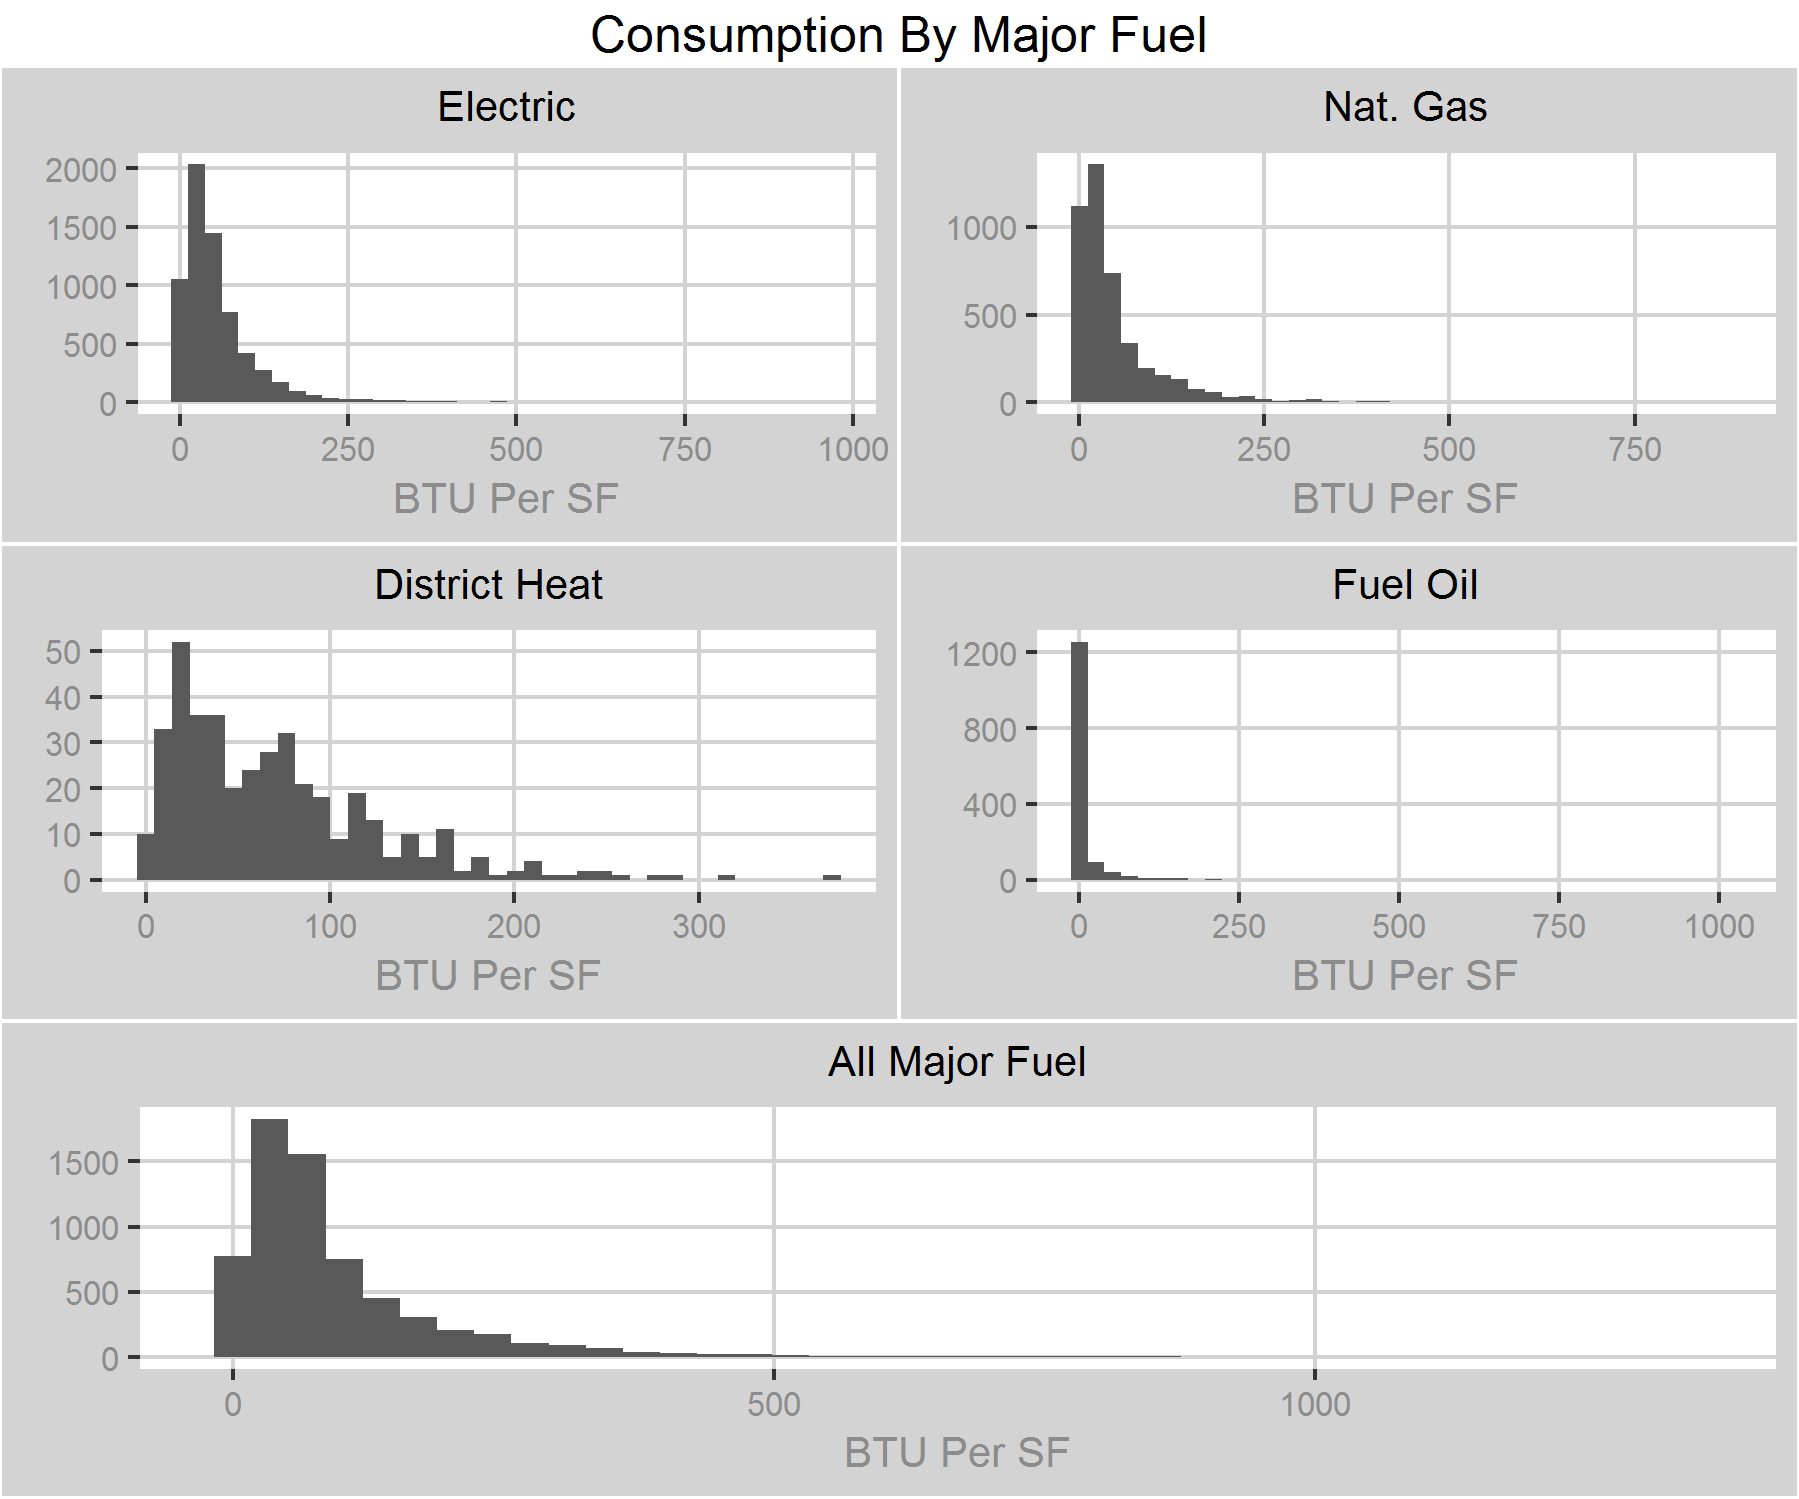
\includegraphics[width=\textwidth]{major_fuels_preliminary_analysis.png}
\centering
\end{figure}

\noindent
{\Large {Objective}}
\\[0.125in]
The goal of this project is two-fold.  First, it is important to explore the data set and determine the influencing factors for each planned response variable.  Second, a predictive model will be constructed for each major fuel consumption type (Electricity, Natural Gas, Fuel Oil, and District Heat, etc.) as well as an additional model for the overall major fuel consumption, which is the sum of the fuel consumption types noted above.  Efforts will be made to explain the model inputs; however, the ultimate goal is the performance of predictions, so some methods may render this goal somewhat incomplete.
\\[0.25in]
{\Large {Deliverable}}
\\[0.125in]
A summary will be provided which will try to explain the domain as well as any major indicators of energy use. Additionally an interface will be provided that can take inputs and provide predictive outputs on anticipated energy consumption.
\end{document}